\documentclass{standalone}
\RequirePackage[table]{xcolor}
\RequirePackage{colortbl}
% Chapters
\definecolor{IBcolCH01}{HTML}{eb3b79}\colorlet{IBcolCH1}{IBcolCH01}
\definecolor{IBcolCH02}{HTML}{9a529f}\colorlet{IBcolCH2}{IBcolCH02}
\definecolor{IBcolCH03}{HTML}{775ba6}\colorlet{IBcolCH3}{IBcolCH03}
\definecolor{IBcolCH04}{HTML}{5a68b0}\colorlet{IBcolCH4}{IBcolCH04}
\definecolor{IBcolCH05}{HTML}{55a0d8}\colorlet{IBcolCH5}{IBcolCH05}
\definecolor{IBcolCH06}{HTML}{34b0e5}\colorlet{IBcolCH6}{IBcolCH06}
\definecolor{IBcolCH07}{HTML}{34c1d7}\colorlet{IBcolCH7}{IBcolCH07}
\definecolor{IBcolCH08}{HTML}{65bc6a}\colorlet{IBcolCH8}{IBcolCH08}
\definecolor{IBcolCH09}{HTML}{9acb62}\colorlet{IBcolCH9}{IBcolCH09}
\definecolor{IBcolCH10}{HTML}{d1dd5b}
\definecolor{IBcolCH11}{HTML}{f9ec5d}
\definecolor{IBcolCH12}{HTML}{fbc82a}
\definecolor{IBcolCH13}{HTML}{faa725}
\definecolor{IBcolCH14}{HTML}{f26f47}
\definecolor{IBcolCH15}{HTML}{8e6d65}
\definecolor{IBcolCH16}{HTML}{bdbcbc}
\definecolor{IBcolCH17}{HTML}{79919d}
% Learning/definition color
\definecolor{IBcolDef}{HTML}{ef5052}
% Step by step color
\definecolor{IBcolSBS}{HTML}{26a69b}
% Example box color
\definecolor{IBcolEXB}{HTML}{26a69b}
% Cover page
\definecolor{IBcolCOV}{HTML}{073f5c}
\definecolor{IBcolCOV2}{HTML}{3b4d72}
\definecolor{IBcolCOV3}{HTML}{fad155}
\definecolor{IBcolCOV4}{HTML}{1b3b5a}
% Chemistry
\definecolor{IBcolV}{HTML}{26a65b}
\definecolor{IBcolX}{HTML}{a62631}
\usepackage{tikz}
\newcommand{\StudyBuddyTikZ}[1]{\begin{tikzpicture}[y=1pt,x=1pt]
% Book
\fill[#1] (34,480) .. controls ++(20:100) and ++(-25:-80) .. (272,440) -- (272,398) -- (245,403) .. controls ++(90:10) and ++(-25:10) .. (235,432) .. controls ++(-25:-80) and ++(20:100) .. (21,448) .. controls ++(20:-10) and ++(90:5) .. (13,439) -- (13,262) -- (-13,262) --(-13,439) .. controls ++(90:5) and ++(-20:10) .. (-21,448) .. controls ++(-20:-100) and ++(25:80) .. (-235,432) .. controls ++(25:-10) and ++(90:10) .. (-245,403) -- (-272,398) -- (-272,440) .. controls ++(25:80) and ++(-20:-100) .. (-34,480) .. controls ++(25:20) and ++(-25:-20) .. cycle;
% Eyes
\fill[#1] (83,580) circle (29);
\fill[#1] (-83,580) circle (29);
% Hands
\fill[#1] (240,320) circle (58);
\path[fill=white] (240,320) circle (34);
\fill[#1] (-240,320) circle (58);
\path[fill=white] (-240,320) circle (34);
% Head
\fill[#1] (-193,498) -- (-168,506) .. controls (-262,668) and (-133,817) .. (0,817) .. controls (133,817) and (262,668) .. (168,506) -- (193,498) .. controls (237,580) and (232,653) .. (205,710) .. controls (166,793) and (78,842) .. (0,841) .. controls (-78,842) and (-166,793) .. (-205,710) .. controls (-232,653) and (-237,580) .. cycle;
\end{tikzpicture}}
\begin{document}
\begin{tikzpicture}[x=9pt,y=9pt]

    \node[rectangle,text width=50pt,align=center] (Nt1) at (0,  9)   {\strut muscle};
    \node[rectangle,text width=50pt,align=center] (Nb1) at (0, -9)  {\strut cell};
    \node[rectangle,text width=50pt,align=center] (Nt2) at (9,  9)   {\strut cardiac};
    \node[rectangle,text width=50pt,align=center] (Nb2) at (9, -9)  {\strut tissue};
    \node[rectangle,text width=50pt,align=center] (Nt3) at (18, 9)  {\strut heart};
    \node[rectangle,text width=50pt,align=center] (Nb3) at (18,-9) {\strut organ};
    \node[rectangle,text width=50pt,align=center] (Nt4) at (27, 9)  {\strut vascular};
    \node[rectangle,text width=50pt,align=center] (Nb4) at (27,-9) {\strut system};
    \node[rectangle,text width=50pt,align=center] (Nt5) at (36, 9)  {\strut human};
    \node[rectangle,text width=50pt,align=center] (Nb5) at (36,-9) {\strut organism};

    \draw[-latex,line width=2pt] (Nt1.east)--(Nt2.west);
    \draw[-latex,line width=2pt] (Nt2.east)--(Nt3.west);
    \draw[-latex,line width=2pt] (Nt3.east)--(Nt4.west);
    \draw[-latex,line width=2pt] (Nt4.east)--(Nt5.west);

    \draw[-latex,line width=2pt] (Nb1.east)--(Nb2.west);
    \draw[-latex,line width=2pt] (Nb2.east)--(Nb3.west);
    \draw[-latex,line width=2pt] (Nb3.east)--(Nb4.west);
    \draw[-latex,line width=2pt] (Nb4.east)--(Nb5.west);

    % Cell
    \begin{scope}[shift={(0,0)}]
        \fill[IBcolCH11,draw=black] (0,0) circle (1 and 7);
        \fill[IBcolCH13,draw=black] (0,0) circle (0.3 and 1);
    \end{scope}

    % Tissue
    \begin{scope}[shift={(6,0)},scale=0.8]
        %\fill[IBcolCH01] (0,-8) rectangle (8,8);
        \clip (0,-8) rectangle (8,8);
        \foreach \n in {0,...,4} {
            \fill[IBcolCH01,draw=black] ({2*\n},0) circle (1 and 7);
            \fill[IBcolCH13,draw=black] ({2*\n},0) circle (0.3 and 1);

            \fill[IBcolCH01,draw=black] ({2*\n-1},7) circle (1 and 7);
            \fill[IBcolCH13,draw=black] ({2*\n-1},7) circle (0.3 and 1);

            \fill[IBcolCH01,draw=black] ({2*\n-1},-7) circle (1 and 7);
            \fill[IBcolCH13,draw=black] ({2*\n-1},-7) circle (0.3 and 1);
        }
    \end{scope}

% Organ
\node[scale=0.75] at (18,0) {
\begin{tikzpicture}[y=0.80pt, x=0.80pt, yscale=-1.000000, xscale=1.000000, inner sep=0pt, outer sep=0pt]
    \begin{scope}
      \clip
    (369.4633,143.7300) .. controls (353.3347,133.2217) and (353.0683,125.8292) ..
    (355.5737,118.9812) -- (350.2704,117.2135) .. controls (341.3181,137.1374) and
    (326.1371,129.0905) .. (314.4100,139.6894) -- (320.9760,146.7604) .. controls
    (343.1952,135.3054) and (342.8643,149.4074) .. (345.7247,159.8924) .. controls
    (342.8293,187.9542) and (316.8292,217.4163) .. (376.0293,241.7148) .. controls
    (432.9563,236.9261) and (425.6496,166.5670) .. (419.2133,158.8823) .. controls
    (407.5273,148.3752) and (423.1215,141.6970) .. (428.8098,133.6284) --
    (424.7691,126.5574) .. controls (414.7126,131.5200) and (414.2960,123.1350) ..
    (412.6473,116.4559) -- (406.0813,117.2135) .. controls (407.2276,138.5106) and
    (395.6975,133.1870) .. (387.3935,134.6386);
        \fill[IBcolDef!30!white] (300,260) rectangle (450,70);
    \end{scope}
        \begin{scope}
      \clip
    (368.8320,174.1608) .. controls (363.1170,169.6152) and (365.8724,163.7321) ..
    (366.0620,158.2542) .. controls (367.2115,136.2977) and (380.7203,127.7142) ..
    (389.2193,96.2980) -- (397.5971,100.1636) .. controls (378.8037,130.4429) and
    (388.6964,194.9526) .. (376.2818,241.4622);
        \fill[IBcolDef!30!white] (300,260) rectangle (450,70);
    \end{scope}

        \begin{scope}
      \clip
    (382.2165,117.2135) .. controls (375.2227,113.8625) and (373.6755,98.3076) ..
    (373.5897,92.8327) -- (365.9392,92.8423) .. controls (366.0020,105.0271) and
    (366.4640,126.5337) .. (374.5141,131.3556);
        \fill[IBcolDef!30!white] (300,260) rectangle (450,70);
    \end{scope}

  \path[draw=IBcolDef,line join=miter,line cap=butt,line width=2.800pt]
    (382.2165,117.2135) .. controls (375.2227,113.8625) and (373.6755,98.3076) ..
    (373.5897,92.8327) -- (365.9392,92.8423) .. controls (366.0020,105.0271) and
    (366.4640,126.5337) .. (374.5141,131.3556);
  \path[draw=IBcolDef,line join=miter,line cap=butt,line width=2.800pt]
    (368.8320,174.1608) .. controls (363.1170,169.6152) and (365.8724,163.7321) ..
    (366.0620,158.2542) .. controls (367.2115,136.2977) and (380.7203,127.7142) ..
    (389.2193,96.2980) -- (397.5971,100.1636) .. controls (378.8037,130.4429) and
    (388.6964,194.9526) .. (376.2818,241.4622);
  \path[draw=IBcolDef,line join=miter,line cap=butt,line width=2.800pt]
    (369.4633,143.7300) .. controls (353.3347,133.2217) and (353.0683,125.8292) ..
    (355.5737,118.9812) -- (350.2704,117.2135) .. controls (341.3181,137.1374) and
    (326.1371,129.0905) .. (314.4100,139.6894) -- (320.9760,146.7604) .. controls
    (343.1952,135.3054) and (342.8643,149.4074) .. (345.7247,159.8924) .. controls
    (342.8293,187.9542) and (316.8292,217.4163) .. (376.0293,241.7148) .. controls
    (432.9563,236.9261) and (425.6496,166.5670) .. (419.2133,158.8823) .. controls
    (407.5273,148.3752) and (423.1215,141.6970) .. (428.8098,133.6284) --
    (424.7691,126.5574) .. controls (414.7126,131.5200) and (414.2960,123.1350) ..
    (412.6473,116.4559) -- (406.0813,117.2135) .. controls (407.2276,138.5106) and
    (395.6975,133.1870) .. (387.3935,134.6386);
  \path[draw=IBcolDef,line join=miter,line cap=butt,line width=1.800pt]
    (345.8929,159.5050) .. controls (349.8597,159.8414) and (352.3756,163.3119) ..
    (352.1429,172.7193);
  \path[draw=IBcolDef,line join=miter,line cap=butt,line width=1.800pt]
    (367.6786,147.3622) .. controls (373.5607,147.5938) and (379.2827,150.3872) ..
    (385.0000,153.2550);
  \path[draw=IBcolDef,line join=miter,line cap=butt,line width=1.800pt]
    (397.3935,134.1677) .. controls (401.3748,139.0160) and (405.8113,144.7067) ..
    (402.8571,152.3622) .. controls (396.8635,155.0053) and (392.1025,160.0017) ..
    (384.4643,159.5050);
  \path[draw=IBcolDef,line join=miter,line cap=butt,line width=1.800pt]
    (403.2143,152.1836) .. controls (404.8737,157.7625) and (408.3729,162.8021) ..
    (400.7143,171.1122);
  \path[draw=IBcolDef,line join=miter,line cap=butt,line width=1.800pt]
    (418.2143,157.5408) .. controls (414.0324,162.6746) and (410.2769,167.9505) ..
    (413.0357,175.3979);

\end{tikzpicture}
};

% system
\node[scale=0.85] at (27,0) {
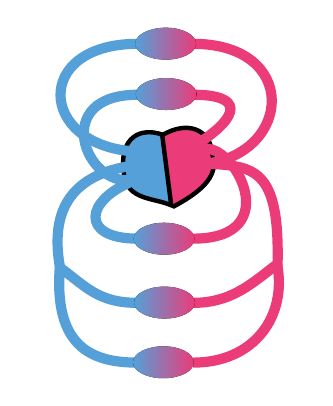
\begin{tikzpicture}[y=0.80pt, x=0.80pt, yscale=-1.000000, xscale=1.000000, inner sep=0pt, outer sep=0pt]
  \path[draw=black,fill=IBcolCH01,line join=miter,line cap=butt,miter
    limit=4.00,line width=1.600pt] (516.2500,137.5408) .. controls
    (528.2648,130.5644) and (536.8285,135.9554) .. (538.2785,143.4804) .. controls
    (538.0227,147.8100) and (546.5242,156.5984) .. (520.9668,169.9885);
  \path[draw=black,fill=IBcolCH05,line join=miter,line cap=butt,miter
    limit=4.00,line width=1.600pt] (516.0714,137.3622) -- (520.1835,169.2940) ..
    controls (511.7326,165.7139) and (500.2496,167.0026) .. (498.7500,155.0408) ..
    controls (496.4280,138.0439) and (506.6236,134.0283) .. (516.0714,137.3622) --
    cycle;
  \path[draw=IBcolCH05,line join=miter,line cap=butt,miter limit=4.00,line
    width=3.680pt] (503.3619,144.9720) .. controls (460.0036,141.9863) and
    (457.6419,96.3622) .. (505.0000,96.3622);
  \path[draw=IBcolCH05,line join=miter,line cap=butt,miter limit=4.00,line
    width=3.680pt] (502.5053,157.7896) .. controls (481.3762,161.2146) and
    (465.3958,119.3622) .. (505.0000,119.3622);
  \path[draw=IBcolCH05,line join=miter,line cap=butt,miter limit=4.00,line
    width=3.680pt] (503.3316,158.2080) .. controls (481.0516,166.8019) and
    (478.7101,184.3622) .. (505.0000,184.3622);
  \path[draw=IBcolCH05,line join=miter,line cap=butt,miter limit=4.00,line
    width=3.680pt] (501.4177,151.5739) .. controls (473.6011,156.1980) and
    (465.4673,173.1147) .. (470.0000,197.7193);
  \path[draw=IBcolCH05,line join=miter,line cap=butt,miter limit=4.00,line
    width=3.680pt] (505.0000,213.3622) .. controls (487.0362,213.3622) and
    (481.5908,205.8790) .. (469.8214,197.3622) .. controls (467.3044,232.0805) and
    (482.9399,240.3622) .. (505.0000,240.3622);
  \path[draw=IBcolCH01,line join=miter,line cap=butt,miter limit=4.00,line
    width=3.680pt] (532.6842,141.1626) .. controls (551.6196,128.6049) and
    (552.6080,119.3622) .. (530.0000,119.3622);
  \path[draw=IBcolCH01,line join=miter,line cap=butt,miter limit=4.00,line
    width=3.680pt] (534.4878,144.0433) .. controls (547.9561,140.0616) and
    (572.8311,184.3622) .. (530.0000,184.3622);
  \path[draw=IBcolCH01,line join=miter,line cap=butt,miter limit=4.00,line
    width=3.680pt] (535.4528,150.6071) .. controls (574.9525,145.6673) and
    (578.1276,96.3622) .. (530.0000,96.3622);
  \path[draw=IBcolCH01,line join=miter,line cap=butt,miter limit=4.00,line
    width=3.680pt] (534.6376,150.3546) .. controls (556.7760,151.7249) and
    (569.1936,150.9610) .. (568.2143,195.7550) .. controls (557.1639,204.0063) and
    (548.0018,213.3622) .. (530.0000,213.3622);
  \path[draw=IBcolCH01,line join=miter,line cap=butt,miter limit=4.00,line
    width=3.680pt] (568.0357,196.1122) .. controls (572.4628,219.2102) and
    (557.8524,240.3622) .. (530.0000,240.3622);
  \fill[left color=IBcolCH05,right color=IBcolCH01,line width=0pt] (531.4106,96.2907)arc(0.012:359.988:13.732053
    and 7.219);
  \fill[shift={(0.214,22.75361)},left color=IBcolCH05,right color=IBcolCH01,line width=0pt]
    (531.4106,96.2907)arc(0.012:359.988:13.732053 and 7.219);
  \fill[shift={(-0.73302,88.09786)},left color=IBcolCH05,right color=IBcolCH01,line width=0pt]
    (531.4106,96.2907)arc(0.012:359.988:13.732053 and 7.219);
  \fill[shift={(-0.54362,116.95034)},left color=IBcolCH05,right color=IBcolCH01,line width=0pt]
    (531.4106,96.2907)arc(0.012:359.988:13.732053 and 7.219);
  \fill[shift={(-1.0487,143.90878)},left color=IBcolCH05,right color=IBcolCH01,line width=0pt]
    (531.4106,96.2907)arc(0.012:359.988:13.732053 and 7.219);
\end{tikzpicture}};

% orgasnism
\node[scale=0.1] at (36,0) {\StudyBuddyTikZ{IBcolDef}};
\end{tikzpicture}
\end{document}